\documentclass[1p]{elsarticle_modified}
%\bibliographystyle{elsarticle-num}

%\usepackage[colorlinks]{hyperref}
%\usepackage{abbrmath_seonhwa} %\Abb, \Ascr, \Acal ,\Abf, \Afrak
\usepackage{amsfonts}
\usepackage{amssymb}
\usepackage{amsmath}
\usepackage{amsthm}
\usepackage{scalefnt}
\usepackage{amsbsy}
\usepackage{kotex}
\usepackage{caption}
\usepackage{subfig}
\usepackage{color}
\usepackage{graphicx}
\usepackage{xcolor} %% white, black, red, green, blue, cyan, magenta, yellow
\usepackage{float}
\usepackage{setspace}
\usepackage{hyperref}

\usepackage{tikz}
\usetikzlibrary{arrows}

\usepackage{multirow}
\usepackage{array} % fixed length table
\usepackage{hhline}

%%%%%%%%%%%%%%%%%%%%%
\makeatletter
\renewcommand*\env@matrix[1][\arraystretch]{%
	\edef\arraystretch{#1}%
	\hskip -\arraycolsep
	\let\@ifnextchar\new@ifnextchar
	\array{*\c@MaxMatrixCols c}}
\makeatother %https://tex.stackexchange.com/questions/14071/how-can-i-increase-the-line-spacing-in-a-matrix
%%%%%%%%%%%%%%%

\usepackage[normalem]{ulem}

\newcommand{\msout}[1]{\ifmmode\text{\sout{\ensuremath{#1}}}\else\sout{#1}\fi}
%SOURCE: \msout is \stkout macro in https://tex.stackexchange.com/questions/20609/strikeout-in-math-mode

\newcommand{\cancel}[1]{
	\ifmmode
	{\color{red}\msout{#1}}
	\else
	{\color{red}\sout{#1}}
	\fi
}

\newcommand{\add}[1]{
	{\color{blue}\uwave{#1}}
}

\newcommand{\replace}[2]{
	\ifmmode
	{\color{red}\msout{#1}}{\color{blue}\uwave{#2}}
	\else
	{\color{red}\sout{#1}}{\color{blue}\uwave{#2}}
	\fi
}

\newcommand{\Sol}{\mathcal{S}} %segment
\newcommand{\D}{D} %diagram
\newcommand{\A}{\mathcal{A}} %arc


%%%%%%%%%%%%%%%%%%%%%%%%%%%%%5 test

\def\sl{\operatorname{\textup{SL}}(2,\Cbb)}
\def\psl{\operatorname{\textup{PSL}}(2,\Cbb)}
\def\quan{\mkern 1mu \triangleright \mkern 1mu}

\theoremstyle{definition}
\newtheorem{thm}{Theorem}[section]
\newtheorem{prop}[thm]{Proposition}
\newtheorem{lem}[thm]{Lemma}
\newtheorem{ques}[thm]{Question}
\newtheorem{cor}[thm]{Corollary}
\newtheorem{defn}[thm]{Definition}
\newtheorem{exam}[thm]{Example}
\newtheorem{rmk}[thm]{Remark}
\newtheorem{alg}[thm]{Algorithm}

\newcommand{\I}{\sqrt{-1}}
\begin{document}

%\begin{frontmatter}
%
%\title{Boundary parabolic representations of knots up to 8 crossings}
%
%%% Group authors per affiliation:
%\author{Yunhi Cho} 
%\address{Department of Mathematics, University of Seoul, Seoul, Korea}
%\ead{yhcho@uos.ac.kr}
%
%
%\author{Seonhwa Kim} %\fnref{s_kim}}
%\address{Center for Geometry and Physics, Institute for Basic Science, Pohang, 37673, Korea}
%\ead{ryeona17@ibs.re.kr}
%
%\author{Hyuk Kim}
%\address{Department of Mathematical Sciences, Seoul National University, Seoul 08826, Korea}
%\ead{hyukkim@snu.ac.kr}
%
%\author{Seokbeom Yoon}
%\address{Department of Mathematical Sciences, Seoul National University, Seoul, 08826,  Korea}
%\ead{sbyoon15@snu.ac.kr}
%
%\begin{abstract}
%We find all boundary parabolic representation of knots up to 8 crossings.
%
%\end{abstract}
%\begin{keyword}
%    \MSC[2010] 57M25 
%\end{keyword}
%
%\end{frontmatter}

%\linenumbers
%\tableofcontents
%
\newcommand\colored[1]{\textcolor{white}{\rule[-0.35ex]{0.8em}{1.4ex}}\kern-0.8em\color{red} #1}%
%\newcommand\colored[1]{\textcolor{white}{ #1}\kern-2.17ex	\textcolor{white}{ #1}\kern-1.81ex	\textcolor{white}{ #1}\kern-2.15ex\color{red}#1	}

{\Large $\underline{11a_{68}~(K11a_{68})}$}

\setlength{\tabcolsep}{10pt}
\renewcommand{\arraystretch}{1.6}
\vspace{1cm}\begin{tabular}{m{100pt}>{\centering\arraybackslash}m{274pt}}
\multirow{5}{120pt}{
	\centering
	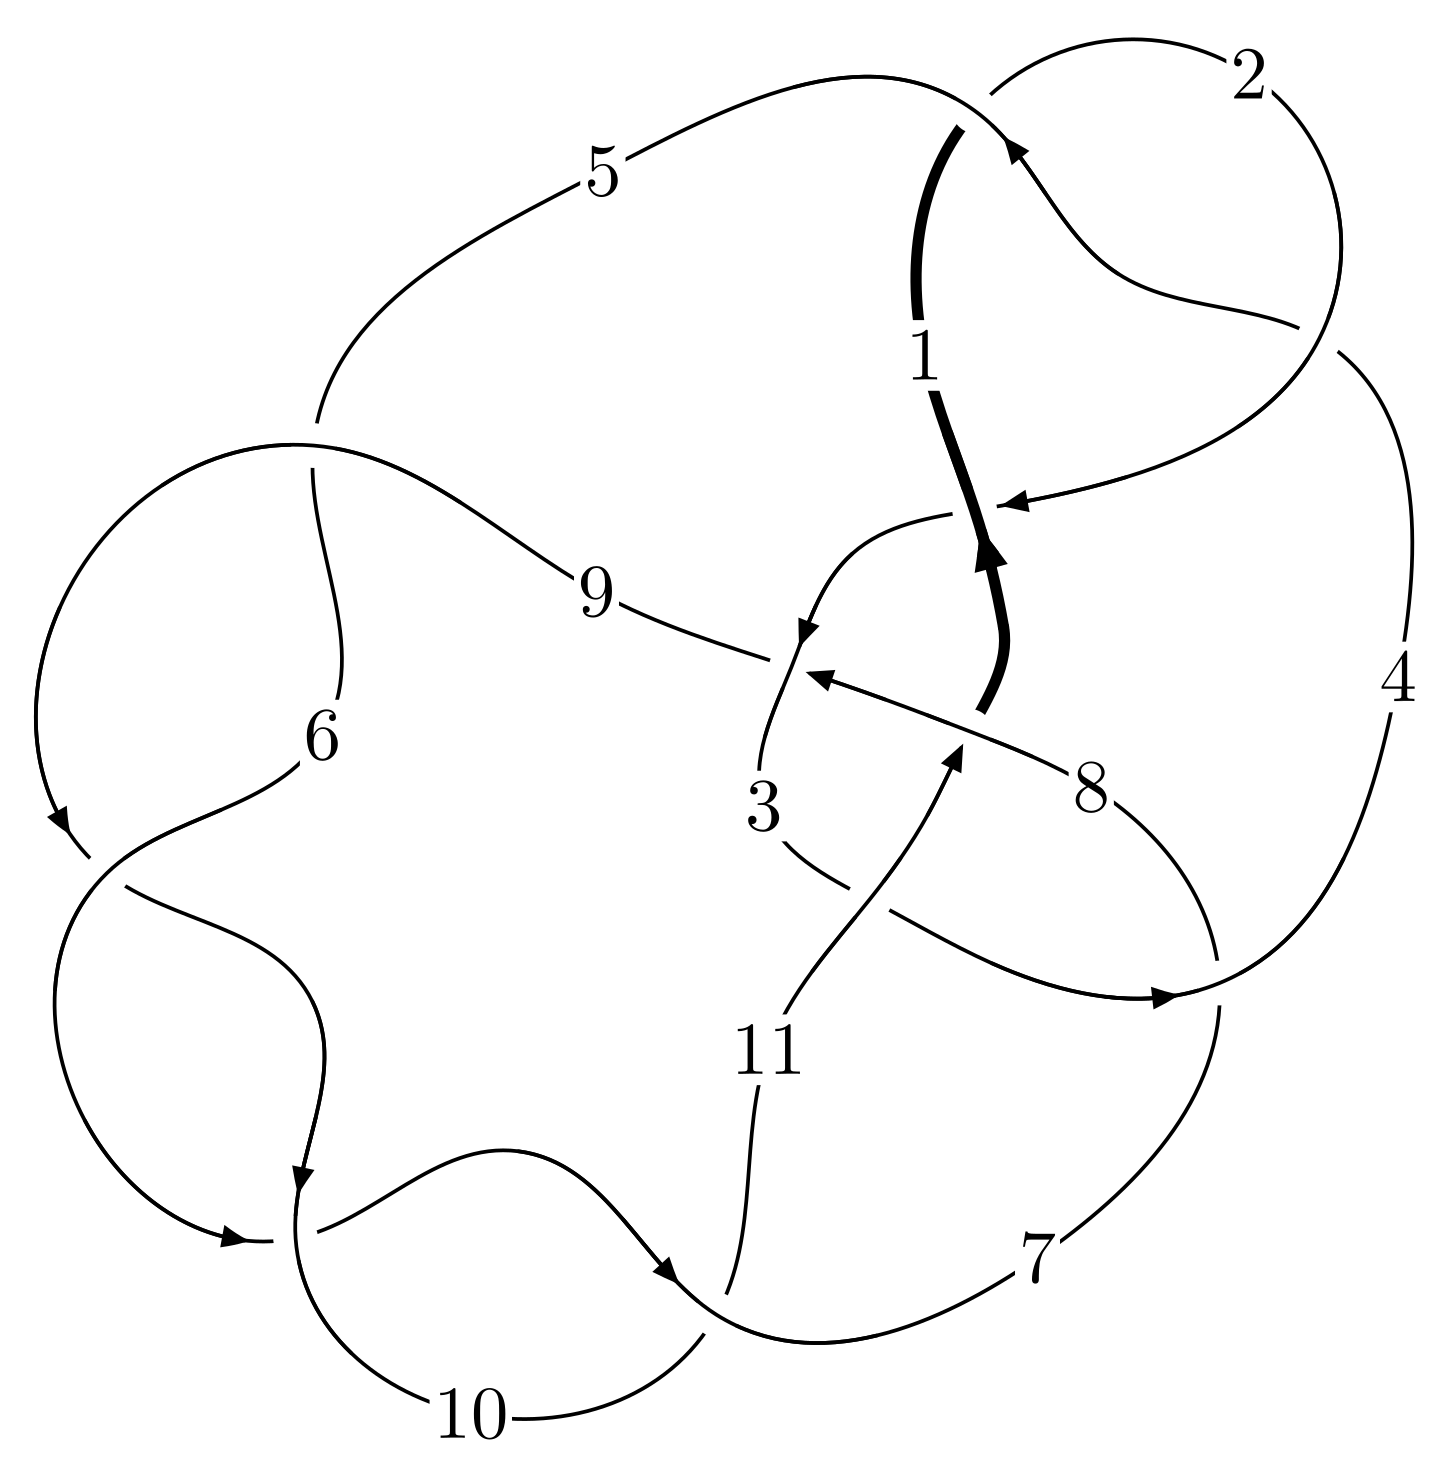
\includegraphics[width=112pt]{../../../GIT/diagram.site/Diagrams/png/317_11a_68.png}\\
\ \ \ A knot diagram\footnotemark}&
\allowdisplaybreaks
\textbf{Linearized knot diagam} \\
\cline{2-2}
 &
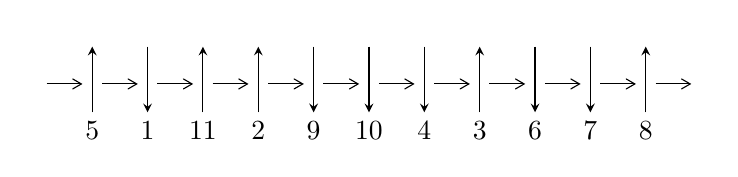
\begin{tikzpicture}[x=20pt, y=17pt]
	% nodes
	\node (C0) at (0, 0) {};
	\node (C1) at (1, 0) {};
	\node (C1U) at (1, +1) {};
	\node (C1D) at (1, -1) {5};

	\node (C2) at (2, 0) {};
	\node (C2U) at (2, +1) {};
	\node (C2D) at (2, -1) {1};

	\node (C3) at (3, 0) {};
	\node (C3U) at (3, +1) {};
	\node (C3D) at (3, -1) {11};

	\node (C4) at (4, 0) {};
	\node (C4U) at (4, +1) {};
	\node (C4D) at (4, -1) {2};

	\node (C5) at (5, 0) {};
	\node (C5U) at (5, +1) {};
	\node (C5D) at (5, -1) {9};

	\node (C6) at (6, 0) {};
	\node (C6U) at (6, +1) {};
	\node (C6D) at (6, -1) {10};

	\node (C7) at (7, 0) {};
	\node (C7U) at (7, +1) {};
	\node (C7D) at (7, -1) {4};

	\node (C8) at (8, 0) {};
	\node (C8U) at (8, +1) {};
	\node (C8D) at (8, -1) {3};

	\node (C9) at (9, 0) {};
	\node (C9U) at (9, +1) {};
	\node (C9D) at (9, -1) {6};

	\node (C10) at (10, 0) {};
	\node (C10U) at (10, +1) {};
	\node (C10D) at (10, -1) {7};

	\node (C11) at (11, 0) {};
	\node (C11U) at (11, +1) {};
	\node (C11D) at (11, -1) {8};
	\node (C12) at (12, 0) {};

	% arrows
	\draw[->,>={angle 60}]
	(C0) edge (C1) (C1) edge (C2) (C2) edge (C3) (C3) edge (C4) (C4) edge (C5) (C5) edge (C6) (C6) edge (C7) (C7) edge (C8) (C8) edge (C9) (C9) edge (C10) (C10) edge (C11) (C11) edge (C12) ;	\draw[->,>=stealth]
	(C1D) edge (C1U) (C2U) edge (C2D) (C3D) edge (C3U) (C4D) edge (C4U) (C5U) edge (C5D) (C6U) edge (C6D) (C7U) edge (C7D) (C8D) edge (C8U) (C9U) edge (C9D) (C10U) edge (C10D) (C11D) edge (C11U) ;
	\end{tikzpicture} \\
\hhline{~~} \\& 
\textbf{Solving Sequence} \\ \cline{2-2} 
 &
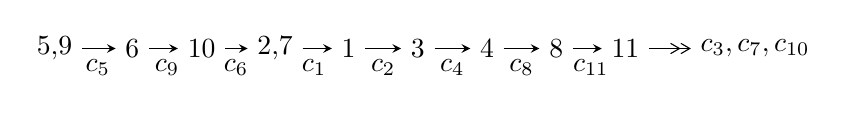
\begin{tikzpicture}[x=25pt, y=7pt]
	% node
	\node (A0) at (-1/8, 0) {5,9};
	\node (A1) at (1, 0) {6};
	\node (A2) at (2, 0) {10};
	\node (A3) at (49/16, 0) {2,7};
	\node (A4) at (33/8, 0) {1};
	\node (A5) at (41/8, 0) {3};
	\node (A6) at (49/8, 0) {4};
	\node (A7) at (57/8, 0) {8};
	\node (A8) at (65/8, 0) {11};
	\node (C1) at (1/2, -1) {$c_{5}$};
	\node (C2) at (3/2, -1) {$c_{9}$};
	\node (C3) at (5/2, -1) {$c_{6}$};
	\node (C4) at (29/8, -1) {$c_{1}$};
	\node (C5) at (37/8, -1) {$c_{2}$};
	\node (C6) at (45/8, -1) {$c_{4}$};
	\node (C7) at (53/8, -1) {$c_{8}$};
	\node (C8) at (61/8, -1) {$c_{11}$};
	\node (A9) at (10, 0) {$c_{3},c_{7},c_{10}$};

	% edge
	\draw[->,>=stealth]	
	(A0) edge (A1) (A1) edge (A2) (A2) edge (A3) (A3) edge (A4) (A4) edge (A5) (A5) edge (A6) (A6) edge (A7) (A7) edge (A8) ;
	\draw[->>,>={angle 60}]	
	(A8) edge (A9);
\end{tikzpicture} \\ 

\end{tabular} \\

\footnotetext{
The image of knot diagram is generated by the software ``\textbf{Draw programme}" developed by Andrew Bartholomew(\url{http://www.layer8.co.uk/maths/draw/index.htm\#Running-draw}), where we modified some parts for our purpose(\url{https://github.com/CATsTAILs/LinksPainter}).
}\phantom \\ \newline 
\centering \textbf{Ideals for irreducible components\footnotemark of $X_{\text{par}}$} 
 
\begin{align*}
I^u_{1}&=\langle 
1.33754\times10^{33} u^{52}-3.23197\times10^{33} u^{51}+\cdots+3.06100\times10^{33} b-5.79603\times10^{32},\\
\phantom{I^u_{1}}&\phantom{= \langle  }2.88344\times10^{33} u^{52}-6.19301\times10^{33} u^{51}+\cdots+1.53050\times10^{33} a+5.13286\times10^{33},\;u^{53}-3 u^{52}+\cdots-2 u-1\rangle \\
I^u_{2}&=\langle 
2 b- a-1,\;a^2+3,\;u-1\rangle \\
\\
\end{align*}
\raggedright * 2 irreducible components of $\dim_{\mathbb{C}}=0$, with total 55 representations.\\
\footnotetext{All coefficients of polynomials are rational numbers. But the coefficients are sometimes approximated in decimal forms when there is not enough margin.}
\newpage
\renewcommand{\arraystretch}{1}
\centering \section*{I. $I^u_{1}= \langle 1.34\times10^{33} u^{52}-3.23\times10^{33} u^{51}+\cdots+3.06\times10^{33} b-5.80\times10^{32},\;2.88\times10^{33} u^{52}-6.19\times10^{33} u^{51}+\cdots+1.53\times10^{33} a+5.13\times10^{33},\;u^{53}-3 u^{52}+\cdots-2 u-1 \rangle$}
\flushleft \textbf{(i) Arc colorings}\\
\begin{tabular}{m{7pt} m{180pt} m{7pt} m{180pt} }
\flushright $a_{5}=$&$\begin{pmatrix}1\\0\end{pmatrix}$ \\
\flushright $a_{9}=$&$\begin{pmatrix}0\\u\end{pmatrix}$ \\
\flushright $a_{6}=$&$\begin{pmatrix}1\\u^2\end{pmatrix}$ \\
\flushright $a_{10}=$&$\begin{pmatrix}- u\\- u^3+u\end{pmatrix}$ \\
\flushright $a_{2}=$&$\begin{pmatrix}-1.88398 u^{52}+4.04640 u^{51}+\cdots-10.2306 u-3.35372\\-0.436961 u^{52}+1.05586 u^{51}+\cdots+2.97372 u+0.189351\end{pmatrix}$ \\
\flushright $a_{7}=$&$\begin{pmatrix}- u^2+1\\- u^4+2 u^2\end{pmatrix}$ \\
\flushright $a_{1}=$&$\begin{pmatrix}-1.44702 u^{52}+2.99054 u^{51}+\cdots-13.2043 u-3.54307\\-0.436961 u^{52}+1.05586 u^{51}+\cdots+2.97372 u+0.189351\end{pmatrix}$ \\
\flushright $a_{3}=$&$\begin{pmatrix}7.03077 u^{52}-17.2162 u^{51}+\cdots+48.9314 u+11.3527\\-0.134450 u^{52}+0.381432 u^{51}+\cdots+3.81964 u+1.58483\end{pmatrix}$ \\
\flushright $a_{4}=$&$\begin{pmatrix}-7.77919 u^{52}+19.0017 u^{51}+\cdots-53.0234 u-12.7464\\0.270228 u^{52}-0.655751 u^{51}+\cdots-3.43986 u-1.30077\end{pmatrix}$ \\
\flushright $a_{8}=$&$\begin{pmatrix}-4.90683 u^{52}+11.3667 u^{51}+\cdots-31.5879 u-8.19442\\-0.449321 u^{52}+0.286138 u^{51}+\cdots+3.58531 u+0.111845\end{pmatrix}$ \\
\flushright $a_{11}=$&$\begin{pmatrix}u^3-2 u\\u^5-3 u^3+u\end{pmatrix}$\\ \flushright $a_{11}=$&$\begin{pmatrix}u^3-2 u\\u^5-3 u^3+u\end{pmatrix}$\\&\end{tabular}
\flushleft \textbf{(ii) Obstruction class $= -1$}\\~\\
\flushleft \textbf{(iii) Cusp Shapes $= 44.2881 u^{52}-103.441 u^{51}+\cdots+256.874 u+76.5517$}\\~\\
\newpage\renewcommand{\arraystretch}{1}
\flushleft \textbf{(iv) u-Polynomials at the component}\newline \\
\begin{tabular}{m{50pt}|m{274pt}}
Crossings & \hspace{64pt}u-Polynomials at each crossing \\
\hline $$\begin{aligned}c_{1},c_{4}\end{aligned}$$&$\begin{aligned}
&u^{53}+2 u^{52}+\cdots-11 u-1
\end{aligned}$\\
\hline $$\begin{aligned}c_{2}\end{aligned}$$&$\begin{aligned}
&u^{53}+24 u^{52}+\cdots+25 u-1
\end{aligned}$\\
\hline $$\begin{aligned}c_{3}\end{aligned}$$&$\begin{aligned}
&u^{53}+5 u^{52}+\cdots+4 u-4
\end{aligned}$\\
\hline $$\begin{aligned}c_{5},c_{6},c_{9}\\c_{10}\end{aligned}$$&$\begin{aligned}
&u^{53}+3 u^{52}+\cdots-2 u+1
\end{aligned}$\\
\hline $$\begin{aligned}c_{7}\end{aligned}$$&$\begin{aligned}
&u^{53}+2 u^{52}+\cdots-127 u-29
\end{aligned}$\\
\hline $$\begin{aligned}c_{8}\end{aligned}$$&$\begin{aligned}
&u^{53}-20 u^{51}+\cdots+127 u+59
\end{aligned}$\\
\hline $$\begin{aligned}c_{11}\end{aligned}$$&$\begin{aligned}
&u^{53}-3 u^{52}+\cdots-2 u+1
\end{aligned}$\\
\hline
\end{tabular}\\~\\
\newpage\renewcommand{\arraystretch}{1}
\flushleft \textbf{(v) Riley Polynomials at the component}\newline \\
\begin{tabular}{m{50pt}|m{274pt}}
Crossings & \hspace{64pt}Riley Polynomials at each crossing \\
\hline $$\begin{aligned}c_{1},c_{4}\end{aligned}$$&$\begin{aligned}
&y^{53}+24 y^{52}+\cdots+25 y-1
\end{aligned}$\\
\hline $$\begin{aligned}c_{2}\end{aligned}$$&$\begin{aligned}
&y^{53}+12 y^{52}+\cdots+425 y-1
\end{aligned}$\\
\hline $$\begin{aligned}c_{3}\end{aligned}$$&$\begin{aligned}
&y^{53}+15 y^{52}+\cdots+8 y-16
\end{aligned}$\\
\hline $$\begin{aligned}c_{5},c_{6},c_{9}\\c_{10}\end{aligned}$$&$\begin{aligned}
&y^{53}-63 y^{52}+\cdots+8 y-1
\end{aligned}$\\
\hline $$\begin{aligned}c_{7}\end{aligned}$$&$\begin{aligned}
&y^{53}-60 y^{52}+\cdots+14273 y-841
\end{aligned}$\\
\hline $$\begin{aligned}c_{8}\end{aligned}$$&$\begin{aligned}
&y^{53}-40 y^{52}+\cdots-44759 y-3481
\end{aligned}$\\
\hline $$\begin{aligned}c_{11}\end{aligned}$$&$\begin{aligned}
&y^{53}-7 y^{52}+\cdots+8 y-1
\end{aligned}$\\
\hline
\end{tabular}\\~\\
\newpage\flushleft \textbf{(vi) Complex Volumes and Cusp Shapes}
$$\begin{array}{c|c|c}  
\text{Solutions to }I^u_{1}& \I (\text{vol} + \sqrt{-1}CS) & \text{Cusp shape}\\
 \hline 
\begin{aligned}
u &= \phantom{-}0.733711 + 0.645681 I \\
a &= -1.46416 - 1.02659 I \\
b &= \phantom{-}0.413624 - 1.013730 I\end{aligned}
 & -3.39428 - 3.43400 I & \phantom{-0.000000 } 0 \\ \hline\begin{aligned}
u &= \phantom{-}0.733711 - 0.645681 I \\
a &= -1.46416 + 1.02659 I \\
b &= \phantom{-}0.413624 + 1.013730 I\end{aligned}
 & -3.39428 + 3.43400 I & \phantom{-0.000000 } 0 \\ \hline\begin{aligned}
u &= -0.858540 + 0.570989 I \\
a &= -1.30456 + 1.52035 I \\
b &= \phantom{-}0.626693 + 1.121900 I\end{aligned}
 & -2.08339 + 11.83770 I & \phantom{-0.000000 } 0 \\ \hline\begin{aligned}
u &= -0.858540 - 0.570989 I \\
a &= -1.30456 - 1.52035 I \\
b &= \phantom{-}0.626693 - 1.121900 I\end{aligned}
 & -2.08339 - 11.83770 I & \phantom{-0.000000 } 0 \\ \hline\begin{aligned}
u &= -0.890477 + 0.316821 I \\
a &= \phantom{-}0.33516 - 1.62827 I \\
b &= \phantom{-}0.071350 - 1.206910 I\end{aligned}
 & -5.68960 + 3.88038 I & -9.36604 - 5.67169 I \\ \hline\begin{aligned}
u &= -0.890477 - 0.316821 I \\
a &= \phantom{-}0.33516 + 1.62827 I \\
b &= \phantom{-}0.071350 + 1.206910 I\end{aligned}
 & -5.68960 - 3.88038 I & -9.36604 + 5.67169 I \\ \hline\begin{aligned}
u &= -0.790831 + 0.511450 I \\
a &= \phantom{-}0.133210 + 0.424681 I \\
b &= \phantom{-}0.848973 - 0.421707 I\end{aligned}
 & \phantom{-}0.02021 + 6.36572 I & \phantom{-0.000000 } 0. - 6.01738 I \\ \hline\begin{aligned}
u &= -0.790831 - 0.511450 I \\
a &= \phantom{-}0.133210 - 0.424681 I \\
b &= \phantom{-}0.848973 + 0.421707 I\end{aligned}
 & \phantom{-}0.02021 - 6.36572 I & \phantom{-0.000000 -}0. + 6.01738 I \\ \hline\begin{aligned}
u &= \phantom{-}1.042420 + 0.526470 I \\
a &= \phantom{-}0.186261 + 0.817290 I \\
b &= \phantom{-}0.483358 + 1.013930 I\end{aligned}
 & -2.96394 + 2.74414 I & \phantom{-0.000000 } 0 \\ \hline\begin{aligned}
u &= \phantom{-}1.042420 - 0.526470 I \\
a &= \phantom{-}0.186261 - 0.817290 I \\
b &= \phantom{-}0.483358 - 1.013930 I\end{aligned}
 & -2.96394 - 2.74414 I & \phantom{-0.000000 } 0\\
 \hline 
 \end{array}$$\newpage$$\begin{array}{c|c|c}  
\text{Solutions to }I^u_{1}& \I (\text{vol} + \sqrt{-1}CS) & \text{Cusp shape}\\
 \hline 
\begin{aligned}
u &= \phantom{-}1.143820 + 0.277610 I \\
a &= -0.769630 - 1.108100 I \\
b &= \phantom{-}0.398755 - 0.662277 I\end{aligned}
 & -1.68806 - 1.03417 I & \phantom{-0.000000 } 0 \\ \hline\begin{aligned}
u &= \phantom{-}1.143820 - 0.277610 I \\
a &= -0.769630 + 1.108100 I \\
b &= \phantom{-}0.398755 + 0.662277 I\end{aligned}
 & -1.68806 + 1.03417 I & \phantom{-0.000000 } 0 \\ \hline\begin{aligned}
u &= -0.058774 + 0.801973 I \\
a &= -0.804431 - 0.186468 I \\
b &= \phantom{-}0.583629 - 1.059960 I\end{aligned}
 & \phantom{-}0.34476 - 7.28943 I & -1.89770 + 7.29263 I \\ \hline\begin{aligned}
u &= -0.058774 - 0.801973 I \\
a &= -0.804431 + 0.186468 I \\
b &= \phantom{-}0.583629 + 1.059960 I\end{aligned}
 & \phantom{-}0.34476 + 7.28943 I & -1.89770 - 7.29263 I \\ \hline\begin{aligned}
u &= \phantom{-}0.687960 + 0.265512 I \\
a &= -0.675163 - 0.410284 I \\
b &= \phantom{-}0.229892 + 0.048634 I\end{aligned}
 & -1.33343 - 0.48154 I & -6.01943 + 1.63910 I \\ \hline\begin{aligned}
u &= \phantom{-}0.687960 - 0.265512 I \\
a &= -0.675163 + 0.410284 I \\
b &= \phantom{-}0.229892 - 0.048634 I\end{aligned}
 & -1.33343 + 0.48154 I & -6.01943 - 1.63910 I \\ \hline\begin{aligned}
u &= -0.651505 + 0.261966 I \\
a &= \phantom{-}1.01458 - 2.10036 I \\
b &= -0.598899 - 1.150440 I\end{aligned}
 & -0.87805 + 4.69027 I & -3.22278 - 10.95263 I \\ \hline\begin{aligned}
u &= -0.651505 - 0.261966 I \\
a &= \phantom{-}1.01458 + 2.10036 I \\
b &= -0.598899 + 1.150440 I\end{aligned}
 & -0.87805 - 4.69027 I & -3.22278 + 10.95263 I \\ \hline\begin{aligned}
u &= -0.116335 + 0.680396 I \\
a &= -1.030080 + 0.147365 I \\
b &= \phantom{-}0.691596 + 0.477793 I\end{aligned}
 & \phantom{-}2.06084 - 2.35698 I & \phantom{-}2.09384 + 2.25421 I \\ \hline\begin{aligned}
u &= -0.116335 - 0.680396 I \\
a &= -1.030080 - 0.147365 I \\
b &= \phantom{-}0.691596 - 0.477793 I\end{aligned}
 & \phantom{-}2.06084 + 2.35698 I & \phantom{-}2.09384 - 2.25421 I\\
 \hline 
 \end{array}$$\newpage$$\begin{array}{c|c|c}  
\text{Solutions to }I^u_{1}& \I (\text{vol} + \sqrt{-1}CS) & \text{Cusp shape}\\
 \hline 
\begin{aligned}
u &= \phantom{-}0.269726 + 0.624271 I \\
a &= -0.593135 - 0.023709 I \\
b &= \phantom{-}0.209100 + 0.945558 I\end{aligned}
 & -2.15945 - 0.98457 I & -6.47095 + 3.55570 I \\ \hline\begin{aligned}
u &= \phantom{-}0.269726 - 0.624271 I \\
a &= -0.593135 + 0.023709 I \\
b &= \phantom{-}0.209100 - 0.945558 I\end{aligned}
 & -2.15945 + 0.98457 I & -6.47095 - 3.55570 I \\ \hline\begin{aligned}
u &= \phantom{-}0.655763 + 0.086361 I \\
a &= \phantom{-}2.67182 + 5.33529 I \\
b &= -0.482724 + 0.895174 I\end{aligned}
 & -1.15754 - 2.23299 I & \phantom{-}20.7265 - 16.6825 I \\ \hline\begin{aligned}
u &= \phantom{-}0.655763 - 0.086361 I \\
a &= \phantom{-}2.67182 - 5.33529 I \\
b &= -0.482724 - 0.895174 I\end{aligned}
 & -1.15754 + 2.23299 I & \phantom{-}20.7265 + 16.6825 I \\ \hline\begin{aligned}
u &= -0.466397 + 0.273654 I \\
a &= \phantom{-}0.439898 - 0.865824 I \\
b &= -0.801200 - 0.670609 I\end{aligned}
 & \phantom{-}1.29588 + 2.67274 I & \phantom{-}3.47265 - 8.90150 I \\ \hline\begin{aligned}
u &= -0.466397 - 0.273654 I \\
a &= \phantom{-}0.439898 + 0.865824 I \\
b &= -0.801200 + 0.670609 I\end{aligned}
 & \phantom{-}1.29588 - 2.67274 I & \phantom{-}3.47265 + 8.90150 I \\ \hline\begin{aligned}
u &= \phantom{-}0.495853 + 0.132805 I \\
a &= -2.14393 + 2.54599 I \\
b &= -0.437475 - 0.833838 I\end{aligned}
 & -0.90053 + 1.58968 I & -1.24595 - 11.67218 I \\ \hline\begin{aligned}
u &= \phantom{-}0.495853 - 0.132805 I \\
a &= -2.14393 - 2.54599 I \\
b &= -0.437475 + 0.833838 I\end{aligned}
 & -0.90053 - 1.58968 I & -1.24595 + 11.67218 I \\ \hline\begin{aligned}
u &= -0.339540 + 0.303762 I \\
a &= -0.849048 - 0.809276 I \\
b &= -0.694807 + 0.319248 I\end{aligned}
 & \phantom{-}1.60066 - 0.35812 I & \phantom{-}5.75025 - 1.86999 I \\ \hline\begin{aligned}
u &= -0.339540 - 0.303762 I \\
a &= -0.849048 + 0.809276 I \\
b &= -0.694807 - 0.319248 I\end{aligned}
 & \phantom{-}1.60066 + 0.35812 I & \phantom{-}5.75025 + 1.86999 I\\
 \hline 
 \end{array}$$\newpage$$\begin{array}{c|c|c}  
\text{Solutions to }I^u_{1}& \I (\text{vol} + \sqrt{-1}CS) & \text{Cusp shape}\\
 \hline 
\begin{aligned}
u &= \phantom{-}1.56006\phantom{ +0.000000I} \\
a &= -0.846407\phantom{ +0.000000I} \\
b &= -1.04242\phantom{ +0.000000I}\end{aligned}
 & -4.89339\phantom{ +0.000000I} & \phantom{-0.000000 } 0 \\ \hline\begin{aligned}
u &= \phantom{-}1.57394 + 0.03176 I \\
a &= -0.266076 + 0.952973 I \\
b &= -0.981473 + 0.829936 I\end{aligned}
 & -5.77422 - 3.45795 I & \phantom{-0.000000 } 0 \\ \hline\begin{aligned}
u &= \phantom{-}1.57394 - 0.03176 I \\
a &= -0.266076 - 0.952973 I \\
b &= -0.981473 - 0.829936 I\end{aligned}
 & -5.77422 + 3.45795 I & \phantom{-0.000000 } 0 \\ \hline\begin{aligned}
u &= -1.58085 + 0.00270 I \\
a &= -0.420614 + 0.517476 I \\
b &= -0.490850 - 0.618356 I\end{aligned}
 & -8.08310 + 1.37745 I & \phantom{-0.000000 } 0 \\ \hline\begin{aligned}
u &= -1.58085 - 0.00270 I \\
a &= -0.420614 - 0.517476 I \\
b &= -0.490850 + 0.618356 I\end{aligned}
 & -8.08310 - 1.37745 I & \phantom{-0.000000 } 0 \\ \hline\begin{aligned}
u &= \phantom{-}1.60794 + 0.05864 I \\
a &= \phantom{-}0.21792 + 2.23198 I \\
b &= -0.60448 + 1.28732 I\end{aligned}
 & -8.69900 - 5.79684 I & \phantom{-0.000000 } 0 \\ \hline\begin{aligned}
u &= \phantom{-}1.60794 - 0.05864 I \\
a &= \phantom{-}0.21792 - 2.23198 I \\
b &= -0.60448 - 1.28732 I\end{aligned}
 & -8.69900 + 5.79684 I & \phantom{-0.000000 } 0 \\ \hline\begin{aligned}
u &= -1.61440 + 0.12056 I \\
a &= \phantom{-}0.0040355 + 0.1222230 I \\
b &= \phantom{-}0.623522 - 0.278275 I\end{aligned}
 & -9.21922 + 2.19279 I & \phantom{-0.000000 } 0 \\ \hline\begin{aligned}
u &= -1.61440 - 0.12056 I \\
a &= \phantom{-}0.0040355 - 0.1222230 I \\
b &= \phantom{-}0.623522 + 0.278275 I\end{aligned}
 & -9.21922 - 2.19279 I & \phantom{-0.000000 } 0 \\ \hline\begin{aligned}
u &= -1.61997 + 0.02761 I \\
a &= \phantom{-}1.27413 - 2.99101 I \\
b &= -0.490506 - 0.975564 I\end{aligned}
 & -9.14547 + 2.68229 I & \phantom{-0.000000 } 0\\
 \hline 
 \end{array}$$\newpage$$\begin{array}{c|c|c}  
\text{Solutions to }I^u_{1}& \I (\text{vol} + \sqrt{-1}CS) & \text{Cusp shape}\\
 \hline 
\begin{aligned}
u &= -1.61997 - 0.02761 I \\
a &= \phantom{-}1.27413 + 2.99101 I \\
b &= -0.490506 + 0.975564 I\end{aligned}
 & -9.14547 - 2.68229 I & \phantom{-0.000000 } 0 \\ \hline\begin{aligned}
u &= \phantom{-}1.64104 + 0.14587 I \\
a &= \phantom{-}0.552638 - 0.075300 I \\
b &= \phantom{-}0.956160 + 0.388075 I\end{aligned}
 & -8.29591 - 8.86132 I & \phantom{-0.000000 } 0 \\ \hline\begin{aligned}
u &= \phantom{-}1.64104 - 0.14587 I \\
a &= \phantom{-}0.552638 + 0.075300 I \\
b &= \phantom{-}0.956160 - 0.388075 I\end{aligned}
 & -8.29591 + 8.86132 I & \phantom{-0.000000 } 0 \\ \hline\begin{aligned}
u &= -1.64394 + 0.19308 I \\
a &= -0.87986 + 1.71349 I \\
b &= \phantom{-}0.514455 + 1.092180 I\end{aligned}
 & -11.49850 + 6.63397 I & \phantom{-0.000000 } 0 \\ \hline\begin{aligned}
u &= -1.64394 - 0.19308 I \\
a &= -0.87986 - 1.71349 I \\
b &= \phantom{-}0.514455 - 1.092180 I\end{aligned}
 & -11.49850 - 6.63397 I & \phantom{-0.000000 } 0 \\ \hline\begin{aligned}
u &= \phantom{-}1.66296 + 0.08851 I \\
a &= \phantom{-}0.24702 + 2.16359 I \\
b &= \phantom{-}0.098247 + 1.348150 I\end{aligned}
 & -14.5372 - 5.4639 I & \phantom{-0.000000 } 0 \\ \hline\begin{aligned}
u &= \phantom{-}1.66296 - 0.08851 I \\
a &= \phantom{-}0.24702 - 2.16359 I \\
b &= \phantom{-}0.098247 - 1.348150 I\end{aligned}
 & -14.5372 + 5.4639 I & \phantom{-0.000000 } 0 \\ \hline\begin{aligned}
u &= \phantom{-}1.66393 + 0.16732 I \\
a &= -0.72953 - 1.98988 I \\
b &= \phantom{-}0.650090 - 1.173960 I\end{aligned}
 & -10.7030 - 14.7003 I & \phantom{-0.000000 } 0 \\ \hline\begin{aligned}
u &= \phantom{-}1.66393 - 0.16732 I \\
a &= -0.72953 + 1.98988 I \\
b &= \phantom{-}0.650090 + 1.173960 I\end{aligned}
 & -10.7030 + 14.7003 I & \phantom{-0.000000 } 0 \\ \hline\begin{aligned}
u &= -0.111963 + 0.267344 I \\
a &= -0.771605 - 0.811778 I \\
b &= -0.612381 + 0.946401 I\end{aligned}
 & \phantom{-}0.54222 - 2.63785 I & \phantom{-}2.19810 + 0.73658 I\\
 \hline 
 \end{array}$$\newpage$$\begin{array}{c|c|c}  
\text{Solutions to }I^u_{1}& \I (\text{vol} + \sqrt{-1}CS) & \text{Cusp shape}\\
 \hline 
\begin{aligned}
u &= -0.111963 - 0.267344 I \\
a &= -0.771605 + 0.811778 I \\
b &= -0.612381 - 0.946401 I\end{aligned}
 & \phantom{-}0.54222 + 2.63785 I & \phantom{-}2.19810 - 0.73658 I \\ \hline\begin{aligned}
u &= -1.71557 + 0.08761 I \\
a &= \phantom{-}0.04836 - 1.70377 I \\
b &= \phantom{-}0.316553 - 1.065110 I\end{aligned}
 & -12.82680 - 0.50129 I & \phantom{-0.000000 } 0 \\ \hline\begin{aligned}
u &= -1.71557 - 0.08761 I \\
a &= \phantom{-}0.04836 + 1.70377 I \\
b &= \phantom{-}0.316553 + 1.065110 I\end{aligned}
 & -12.82680 + 0.50129 I & \phantom{-0.000000 } 0\\
 \hline 
 \end{array}$$\newpage\newpage\renewcommand{\arraystretch}{1}
\centering \section*{II. $I^u_{2}= \langle 2 b- a-1,\;a^2+3,\;u-1 \rangle$}
\flushleft \textbf{(i) Arc colorings}\\
\begin{tabular}{m{7pt} m{180pt} m{7pt} m{180pt} }
\flushright $a_{5}=$&$\begin{pmatrix}1\\0\end{pmatrix}$ \\
\flushright $a_{9}=$&$\begin{pmatrix}0\\1\end{pmatrix}$ \\
\flushright $a_{6}=$&$\begin{pmatrix}1\\1\end{pmatrix}$ \\
\flushright $a_{10}=$&$\begin{pmatrix}-1\\0\end{pmatrix}$ \\
\flushright $a_{2}=$&$\begin{pmatrix}a\\\frac{1}{2} a+\frac{1}{2}\end{pmatrix}$ \\
\flushright $a_{7}=$&$\begin{pmatrix}0\\1\end{pmatrix}$ \\
\flushright $a_{1}=$&$\begin{pmatrix}\frac{1}{2} a-\frac{1}{2}\\\frac{1}{2} a+\frac{1}{2}\end{pmatrix}$ \\
\flushright $a_{3}=$&$\begin{pmatrix}\frac{1}{2} a-\frac{1}{2}\\\frac{1}{2} a-\frac{1}{2}\end{pmatrix}$ \\
\flushright $a_{4}=$&$\begin{pmatrix}\frac{1}{2} a-\frac{1}{2}\\\frac{1}{2} a-\frac{1}{2}\end{pmatrix}$ \\
\flushright $a_{8}=$&$\begin{pmatrix}\frac{1}{2} a+\frac{1}{2}\\\frac{1}{2} a+\frac{3}{2}\end{pmatrix}$ \\
\flushright $a_{11}=$&$\begin{pmatrix}-1\\-1\end{pmatrix}$\\ \flushright $a_{11}=$&$\begin{pmatrix}-1\\-1\end{pmatrix}$\\&\end{tabular}
\flushleft \textbf{(ii) Obstruction class $= 1$}\\~\\
\flushleft \textbf{(iii) Cusp Shapes $= -2 a-3$}\\~\\
\newpage\renewcommand{\arraystretch}{1}
\flushleft \textbf{(iv) u-Polynomials at the component}\newline \\
\begin{tabular}{m{50pt}|m{274pt}}
Crossings & \hspace{64pt}u-Polynomials at each crossing \\
\hline $$\begin{aligned}c_{1},c_{2}\end{aligned}$$&$\begin{aligned}
&u^2+u+1
\end{aligned}$\\
\hline $$\begin{aligned}c_{3}\end{aligned}$$&$\begin{aligned}
&u^2
\end{aligned}$\\
\hline $$\begin{aligned}c_{4},c_{7},c_{8}\end{aligned}$$&$\begin{aligned}
&u^2- u+1
\end{aligned}$\\
\hline $$\begin{aligned}c_{5},c_{6}\end{aligned}$$&$\begin{aligned}
&(u-1)^2
\end{aligned}$\\
\hline $$\begin{aligned}c_{9},c_{10},c_{11}\end{aligned}$$&$\begin{aligned}
&(u+1)^2
\end{aligned}$\\
\hline
\end{tabular}\\~\\
\newpage\renewcommand{\arraystretch}{1}
\flushleft \textbf{(v) Riley Polynomials at the component}\newline \\
\begin{tabular}{m{50pt}|m{274pt}}
Crossings & \hspace{64pt}Riley Polynomials at each crossing \\
\hline $$\begin{aligned}c_{1},c_{2},c_{4}\\c_{7},c_{8}\end{aligned}$$&$\begin{aligned}
&y^2+y+1
\end{aligned}$\\
\hline $$\begin{aligned}c_{3}\end{aligned}$$&$\begin{aligned}
&y^2
\end{aligned}$\\
\hline $$\begin{aligned}c_{5},c_{6},c_{9}\\c_{10},c_{11}\end{aligned}$$&$\begin{aligned}
&(y-1)^2
\end{aligned}$\\
\hline
\end{tabular}\\~\\
\newpage\flushleft \textbf{(vi) Complex Volumes and Cusp Shapes}
$$\begin{array}{c|c|c}  
\text{Solutions to }I^u_{2}& \I (\text{vol} + \sqrt{-1}CS) & \text{Cusp shape}\\
 \hline 
\begin{aligned}
u &= \phantom{-}1.00000\phantom{ +0.000000I} \\
a &= \phantom{-0.000000 -}1.73205 I \\
b &= \phantom{-}0.500000 + 0.866025 I\end{aligned}
 & -1.64493 + 2.02988 I & -3.00000 - 3.46410 I \\ \hline\begin{aligned}
u &= \phantom{-}1.00000\phantom{ +0.000000I} \\
a &= \phantom{-0.000000 } -1.73205 I \\
b &= \phantom{-}0.500000 - 0.866025 I\end{aligned}
 & -1.64493 - 2.02988 I & -3.00000 + 3.46410 I\\
 \hline 
 \end{array}$$\newpage
\newpage\renewcommand{\arraystretch}{1}
\centering \section*{ III. u-Polynomials}
\begin{tabular}{m{50pt}|m{274pt}}
Crossings & \hspace{64pt}u-Polynomials at each crossing \\
\hline $$\begin{aligned}c_{1}\end{aligned}$$&$\begin{aligned}
&(u^2+u+1)(u^{53}+2 u^{52}+\cdots-11 u-1)
\end{aligned}$\\
\hline $$\begin{aligned}c_{2}\end{aligned}$$&$\begin{aligned}
&(u^2+u+1)(u^{53}+24 u^{52}+\cdots+25 u-1)
\end{aligned}$\\
\hline $$\begin{aligned}c_{3}\end{aligned}$$&$\begin{aligned}
&u^2(u^{53}+5 u^{52}+\cdots+4 u-4)
\end{aligned}$\\
\hline $$\begin{aligned}c_{4}\end{aligned}$$&$\begin{aligned}
&(u^2- u+1)(u^{53}+2 u^{52}+\cdots-11 u-1)
\end{aligned}$\\
\hline $$\begin{aligned}c_{5},c_{6}\end{aligned}$$&$\begin{aligned}
&((u-1)^2)(u^{53}+3 u^{52}+\cdots-2 u+1)
\end{aligned}$\\
\hline $$\begin{aligned}c_{7}\end{aligned}$$&$\begin{aligned}
&(u^2- u+1)(u^{53}+2 u^{52}+\cdots-127 u-29)
\end{aligned}$\\
\hline $$\begin{aligned}c_{8}\end{aligned}$$&$\begin{aligned}
&(u^2- u+1)(u^{53}-20 u^{51}+\cdots+127 u+59)
\end{aligned}$\\
\hline $$\begin{aligned}c_{9},c_{10}\end{aligned}$$&$\begin{aligned}
&((u+1)^2)(u^{53}+3 u^{52}+\cdots-2 u+1)
\end{aligned}$\\
\hline $$\begin{aligned}c_{11}\end{aligned}$$&$\begin{aligned}
&((u+1)^2)(u^{53}-3 u^{52}+\cdots-2 u+1)
\end{aligned}$\\
\hline
\end{tabular}\newpage\renewcommand{\arraystretch}{1}
\centering \section*{ IV. Riley Polynomials}
\begin{tabular}{m{50pt}|m{274pt}}
Crossings & \hspace{64pt}Riley Polynomials at each crossing \\
\hline $$\begin{aligned}c_{1},c_{4}\end{aligned}$$&$\begin{aligned}
&(y^2+y+1)(y^{53}+24 y^{52}+\cdots+25 y-1)
\end{aligned}$\\
\hline $$\begin{aligned}c_{2}\end{aligned}$$&$\begin{aligned}
&(y^2+y+1)(y^{53}+12 y^{52}+\cdots+425 y-1)
\end{aligned}$\\
\hline $$\begin{aligned}c_{3}\end{aligned}$$&$\begin{aligned}
&y^2(y^{53}+15 y^{52}+\cdots+8 y-16)
\end{aligned}$\\
\hline $$\begin{aligned}c_{5},c_{6},c_{9}\\c_{10}\end{aligned}$$&$\begin{aligned}
&((y-1)^2)(y^{53}-63 y^{52}+\cdots+8 y-1)
\end{aligned}$\\
\hline $$\begin{aligned}c_{7}\end{aligned}$$&$\begin{aligned}
&(y^2+y+1)(y^{53}-60 y^{52}+\cdots+14273 y-841)
\end{aligned}$\\
\hline $$\begin{aligned}c_{8}\end{aligned}$$&$\begin{aligned}
&(y^2+y+1)(y^{53}-40 y^{52}+\cdots-44759 y-3481)
\end{aligned}$\\
\hline $$\begin{aligned}c_{11}\end{aligned}$$&$\begin{aligned}
&((y-1)^2)(y^{53}-7 y^{52}+\cdots+8 y-1)
\end{aligned}$\\
\hline
\end{tabular}
\vskip 2pc
\end{document}